% Echoes of Elysium — Graphical Profile
% Spec: docs/brand/spec.md · Compile: xelatex echoes_of_elysium_graphical_profile.tex
\documentclass[11pt,a4paper]{article}

\usepackage[margin=20mm,top=18mm,bottom=20mm]{geometry}
\usepackage{fontspec}
\usepackage{xcolor}
\usepackage{tikz}
\usepackage{graphicx}
\usepackage{booktabs}
\usepackage{tabularx}
\usepackage{enumitem}
\usepackage{hyperref}
\usepackage{fancyhdr}
\usepackage{titlesec}
\usepackage{setspace}

\graphicspath{{../../assets/icon/}}

% —— Foundations ——————————————————————————————————————————————————
\definecolor{voidink}{HTML}{06060F}
\definecolor{panel}{HTML}{141422}
\definecolor{panelsoft}{HTML}{1C1C2E}
\definecolor{ghost}{HTML}{F2F4FA}
\definecolor{muted}{HTML}{B4B8CC}
\definecolor{meta}{HTML}{D2D6E6}
\definecolor{ink}{HTML}{0A0A14}

% —— Exactly 3 accent colours (spec) ——————————————————————————————
\definecolor{signal}{HTML}{00FFCC}   % Accent 1 — Signal Teal
\definecolor{glimmer}{HTML}{FFE08A}  % Accent 2 — Glimmer Gold
\definecolor{pulse}{HTML}{AA44FF}    % Accent 3 — Pulse Violet

% —— Exactly 2 typefaces (spec) ———————————————————————————————————
\setmainfont{DejaVu Sans}[Ligatures=TeX]
\setsansfont{Comfortaa}[
  Path=/usr/share/fonts/truetype/comfortaa/,
  UprightFont=Comfortaa-Regular.ttf,
  BoldFont=Comfortaa-Bold.ttf,
]
\setmonofont{DejaVu Sans Mono}[Scale=0.95]

\newfontfamily\titlefont{Comfortaa}[
  Path=/usr/share/fonts/truetype/comfortaa/,
  UprightFont=Comfortaa-Bold.ttf,
  BoldFont=Comfortaa-Bold.ttf,
  LetterSpace=2,
]
\newfontfamily\markfont{Comfortaa}[
  Path=/usr/share/fonts/truetype/comfortaa/,
  UprightFont=Comfortaa-Bold.ttf,
  BoldFont=Comfortaa-Bold.ttf,
  LetterSpace=6,
]
\newfontfamily\labelfont{DejaVu Sans}[LetterSpace=2]

\pagecolor{voidink}
\color{ghost}
\hypersetup{
  colorlinks=true,
  linkcolor=signal,
  urlcolor=glimmer,
  pdfauthor={Echoes of Elysium},
  pdftitle={Echoes of Elysium — Graphical Profile},
  pdfsubject={Visual identity · spec.md},
}

\pagestyle{fancy}
\fancyhf{}
\renewcommand{\headrulewidth}{0pt}
\renewcommand{\footrulewidth}{0.4pt}
\renewcommand{\footrule}{\hbox to\headwidth{\color{signal!50}\leaders\hrule height \footrulewidth\hfill}}
\fancyfoot[L]{\footnotesize\textcolor{muted}{\labelfont ECHOES OF ELYSIUM · GRAPHICAL PROFILE}}
\fancyfoot[R]{\footnotesize\textcolor{meta}{\thepage}}

\titleformat{\section}
  {\titlefont\Large}{\thesection}{0.8em}{}
  [{\vspace{-0.35em}\color{signal!65}\hrule height 0.55pt}]
\titleformat{\subsection}
  {\sffamily\bfseries\large\color{glimmer}}{\thesubsection}{0.55em}{}

\setlist[itemize]{leftmargin=1.4em, itemsep=0.3em, topsep=0.45em}
\setstretch{1.3}
\setlength{\parskip}{0.3em}

\newcommand{\hex}[1]{\texttt{\##1}}
\newcommand{\keylabel}[1]{\textcolor{signal}{\textbf{#1}}}

% Accent swatch: colour field + dark plate with hex/rgb/hsl
\newcommand{\accentswatch}[5]{%
  \begin{tikzpicture}
    \fill[#1] (0,1.15) rectangle (5.4,2.55);
    \fill[panelsoft] (0,0) rectangle (5.4,1.15);
    \draw[ghost!40, line width=0.5pt] (0,0) rectangle (5.4,2.55);
    \node[anchor=north west, inner sep=6pt, font=\sffamily\bfseries]
          at (0,1.15) {\textcolor{ghost}{#2}};
    \node[anchor=north west, inner sep=6pt, align=left]
          at (0,0.72) {%
      \textcolor{ghost}{\ttfamily\small\##3}\\[0.15em]
      \textcolor{meta}{\ttfamily\footnotesize rgb(#4)}\\[0.1em]
      \textcolor{muted}{\ttfamily\footnotesize hsl(#5)}%
    };
  \end{tikzpicture}%
}

\begin{document}
\thispagestyle{empty}

% =====================================================================
% COVER
% =====================================================================
\vspace*{2.2cm}
\begin{center}
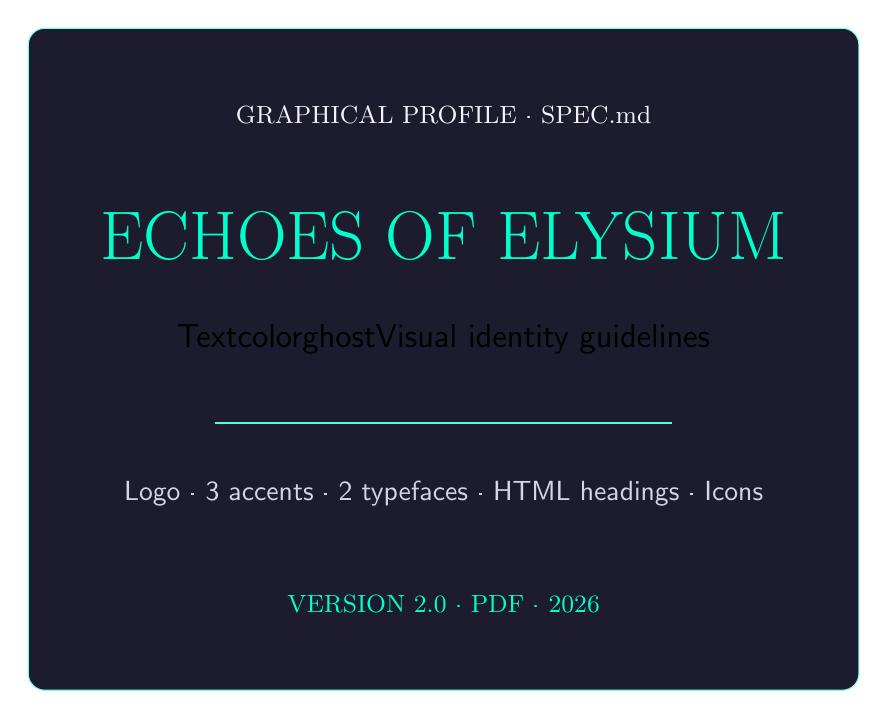
\begin{tikzpicture}
  \node[fill=panelsoft, draw=signal!50, rounded corners=6pt,
        inner xsep=26pt, inner ysep=28pt, align=center] {
    {\textcolor{ghost}{\labelfont\small GRAPHICAL PROFILE · SPEC.md}}\\[1.1cm]
    {\textcolor{signal}{\markfont\Huge ECHOES OF ELYSIUM}}\\[0.7cm]
    {\sffamily\large Textcolor{ghost}{Visual identity guidelines}}\\[0.55cm]
    {\textcolor{signal!70}{\rule{5.8cm}{0.65pt}}}\\[0.55cm]
    {\sffamily\textcolor{meta}{Logo · 3 accents · 2 typefaces · HTML headings · Icons}}\\[1.0cm]
    {\textcolor{signal}{\labelfont\small VERSION 2.0 · PDF · 2026}}
  };
\end{tikzpicture}
\end{center}

\vspace{1.4cm}
\begin{center}
{\sffamily\small\textcolor{muted}{Deliverable format: \textbf{\textcolor{ghost}{.pdf}} (this file)}}
\end{center}

\clearpage

% =====================================================================
% SPEC CHECKLIST
% =====================================================================
\section*{00 · Spec checklist}
\addcontentsline{toc}{section}{Spec checklist}

This profile answers every item in \texttt{docs/brand/spec.md}:

\begin{enumerate}
  \item Logo / application icon on \textbf{black} and \textbf{white} grounds
  \item \textbf{3} accent colours — HEX, RGB, and HSL
  \item \textbf{2} typefaces
  \item Sizes for all HTML heading tags (\texttt{h1}--\texttt{h6})
  \item Icon package
  \item File format: \textbf{PDF}
\end{enumerate}

\clearpage

% =====================================================================
% 1. LOGO / APP ICON
% =====================================================================
\section*{01 · Logotyp \& applikationsikon}
\addcontentsline{toc}{section}{Logotyp \& applikationsikon}

Primary mark: \textbf{app icon} (\texttt{assets/icon/app\_icon.png}) plus the Comfortaa wordmark.
The icon must remain readable as a launcher tile on both dark and light system chrome.

\vspace{0.7em}
\subsection*{On black (default / dark UI)}
\begin{center}
\begin{tikzpicture}
  \fill[voidink] (0,0) rectangle (7.2,5.2);
  \draw[ghost!25] (0,0) rectangle (7.2,5.2);
  \node at (3.6,3.15) {
\includegraphics[width=2.6cm]{app_icon.png}};
  \node[font=\markfont\large, text=signal] at (3.6,1.15) {ECHOES OF ELYSIUM};
  \node[font=\ttfamily\footnotesize, text=muted] at (3.6,0.45) {Preferred · dark ground};
\end{tikzpicture}
\end{center}

\vspace{0.8em}
\subsection*{On white (light / print / lock screen)}
\begin{center}
\begin{tikzpicture}
  \fill[ghost] (0,0) rectangle (7.2,5.2);
  \draw[ink!15] (0,0) rectangle (7.2,5.2);
  \node at (3.6,3.15) {
\includegraphics[width=2.6cm]{app_icon.png}};
  \node[font=\sffamily\bfseries\large, text=ink] at (3.6,1.15) {ECHOES OF ELYSIUM};
  \node[font=\ttfamily\footnotesize, text=ink!55] at (3.6,0.45) {Light ground · ink wordmark};
\end{tikzpicture}
\end{center}

\vspace{0.7em}
\subsection*{Rules}
\begin{itemize}
  \item Keep clear space $\ge$ 12\% of icon width on all sides.
  \item Do not recolour the icon art; place it on solid black or white only.
  \item On light grounds, set the wordmark in Void Ink \hex{06060F} — never Signal Teal on white for long titles.
  \item Source: \texttt{assets/icon/app\_icon.png} (512$\times$512). Generated launcher assets via \texttt{flutter\_launcher\_icons}.
\end{itemize}

\clearpage

% =====================================================================
% 2. THREE ACCENTS
% =====================================================================
\section*{02 · Accent colours (3)}
\addcontentsline{toc}{section}{Accent colours}

Exactly \textbf{three} brand accents. Each lists HEX, RGB, and HSL. Foundations (Void Ink / Panel / Ghost) are staging colours, not accents.

\vspace{0.55em}
\begin{center}
\accentswatch{signal}{1 · Signal Teal}{00FFCC}{0, 255, 204}{168°, 100\%, 50\%}
\hspace{0.35em}
\accentswatch{glimmer}{2 · Glimmer Gold}{FFE08A}{255, 224, 138}{44°, 100\%, 77\%}
\end{center}

\vspace{0.55em}
\begin{center}
\accentswatch{pulse}{3 · Pulse Violet}{AA44FF}{170, 68, 255}{273°, 100\%, 63\%}
\end{center}

\vspace{0.85em}
\renewcommand{\arraystretch}{1.4}
{\small
\begin{tabularx}{\textwidth}{@{}l >{\ttfamily}l >{\ttfamily}l >{\ttfamily}X@{}}
  \toprule
  \textcolor{signal}{\sffamily\bfseries Name} &
  \textcolor{signal}{\sffamily\bfseries Hex} &
  \textcolor{signal}{\sffamily\bfseries RGB} &
  \textcolor{signal}{\sffamily\bfseries HSL} \\
  \midrule
  \sffamily Signal Teal & \#00FFCC & 0,\,255,\,204 & 168°,\,100\%,\,50\% \\
  \sffamily Glimmer Gold & \#FFE08A & 255,\,224,\,138 & 44°,\,100\%,\,77\% \\
  \sffamily Pulse Violet & \#AA44FF & 170,\,68,\,255 & 273°,\,100\%,\,63\% \\
  \bottomrule
\end{tabularx}}
\renewcommand{\arraystretch}{1}

\vspace{0.75em}
\subsection*{Usage}
\begin{itemize}
  \item \textbf{Signal Teal} — primary UI chrome, titles, confirms, Phase.
  \item \textbf{Glimmer Gold} — XP, currency, secondary highlights.
  \item \textbf{Pulse Violet} — special abilities (Pulse / Anchor), Gaia-adjacent cues.
\end{itemize}

\clearpage

% =====================================================================
% 3. TWO FONTS
% =====================================================================
\section*{03 · Typefaces (2)}
\addcontentsline{toc}{section}{Typefaces}

Exactly \textbf{two} faces:

\vspace{0.5em}
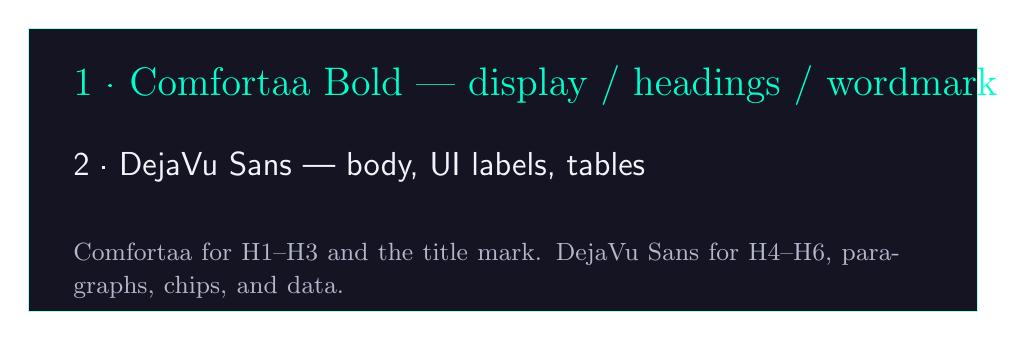
\begin{tikzpicture}
  \fill[panel] (0,0) rectangle (\textwidth-2pt,3.6);
  \draw[signal!40] (0,0) rectangle (\textwidth-2pt,3.6);
  \node[anchor=north west] at (0.45,3.25)
    {\textcolor{signal}{\titlefont\Large 1 · Comfortaa Bold — display / headings / wordmark}};
  \node[anchor=north west] at (0.45,2.15)
    {\textcolor{ghost}{\sffamily\large 2 · DejaVu Sans — body, UI labels, tables}};
  \node[anchor=north west, text width=\textwidth-1.3cm] at (0.45,1.0)
    {\textcolor{muted}{\small Comfortaa for H1--H3 and the title mark. DejaVu Sans for H4--H6, paragraphs, chips, and data.}};
\end{tikzpicture}

\vspace{0.8em}
\renewcommand{\arraystretch}{1.35}
\begin{tabularx}{\textwidth}{@{}l l X@{}}
  \toprule
  \textcolor{signal}{Role} & \textcolor{signal}{Face} & \textcolor{signal}{Notes} \\
  \midrule
  Display & Comfortaa Bold & Wordmark, section titles, H1--H3 \\
  UI / body & DejaVu Sans & H4--H6, copy, HUD chips, forms \\
  \bottomrule
\end{tabularx}
\renewcommand{\arraystretch}{1}

\clearpage

% =====================================================================
% 4. HTML HEADING SIZES
% =====================================================================
\section*{04 · HTML heading sizes}
\addcontentsline{toc}{section}{HTML heading sizes}

Root: \texttt{html \{ font-size: 16px; \}} — sizes below are for \texttt{h1}--\texttt{h6}.
Comfortaa for H1--H3; DejaVu Sans for H4--H6.

\vspace{0.55em}
\renewcommand{\arraystretch}{1.45}
{\small
\begin{tabularx}{\textwidth}{@{}l l l l X@{}}
  \toprule
  \textcolor{signal}{\textbf{Tag}} &
  \textcolor{signal}{\textbf{Size}} &
  \textcolor{signal}{\textbf{rem}} &
  \textcolor{signal}{\textbf{Weight}} &
  \textcolor{signal}{\textbf{Face / tracking}} \\
  \midrule
  \texttt{h1} & 40\,px & 2.5\,rem & 700 & Comfortaa · letter-spacing 0.04em \\
  \texttt{h2} & 32\,px & 2.0\,rem & 700 & Comfortaa · 0.03em \\
  \texttt{h3} & 24\,px & 1.5\,rem & 700 & Comfortaa · 0.02em \\
  \texttt{h4} & 20\,px & 1.25\,rem & 700 & DejaVu Sans \\
  \texttt{h5} & 16\,px & 1.0\,rem & 700 & DejaVu Sans \\
  \texttt{h6} & 14\,px & 0.875\,rem & 700 & DejaVu Sans · uppercase OK · 0.08em \\
  \bottomrule
\end{tabularx}}
\renewcommand{\arraystretch}{1}

\vspace{0.9em}
\subsection*{Specimen}
{\titlefont\Huge H1 · Echoes of Elysium}\\[0.25em]
{\titlefont\Large H2 · Colony forests}\\[0.2em]
{\titlefont\large H3 · Signal lock}\\[0.2em]
{\sffamily\bfseries\large H4 · Mission brief}\\[0.15em]
{\sffamily\bfseries H5 · Status line}\\[0.15em]
{\sffamily\bfseries\small H6 · MENU · PHASE · WARD}

\vspace{0.7em}
\subsection*{CSS sketch}
\begin{verbatim}
h1 { font-family: Comfortaa, sans-serif; font-size: 2.5rem;  font-weight: 700; letter-spacing: 0.04em; }
h2 { font-family: Comfortaa, sans-serif; font-size: 2.0rem;  font-weight: 700; letter-spacing: 0.03em; }
h3 { font-family: Comfortaa, sans-serif; font-size: 1.5rem;  font-weight: 700; letter-spacing: 0.02em; }
h4 { font-family: "DejaVu Sans", system-ui, sans-serif; font-size: 1.25rem; font-weight: 700; }
h5 { font-family: "DejaVu Sans", system-ui, sans-serif; font-size: 1.0rem;  font-weight: 700; }
h6 { font-family: "DejaVu Sans", system-ui, sans-serif; font-size: 0.875rem; font-weight: 700; letter-spacing: 0.08em; }
\end{verbatim}

\clearpage

% =====================================================================
% 5. ICONS
% =====================================================================
\section*{05 · Ikonpaket}
\addcontentsline{toc}{section}{Ikonpaket}

\begin{itemize}
  \item \textbf{Package:} Flutter \textbf{Material Icons} (\texttt{Icons.*} from \texttt{package:flutter/material.dart})
  \item \textbf{Declared:} \texttt{cupertino\_icons: \^{}1.0.2} in \texttt{pubspec.yaml} (available; UI currently uses Material)
  \item \textbf{Usage:} outlined where possible (\texttt{Icons.close}, \texttt{Icons.menu}, \texttt{Icons.lock\_outline}, \texttt{Icons.storefront\_outlined}, \ldots)
  \item \textbf{Style:} single-colour glyphs tinted with Ghost / accents — no multicolour icons in chrome
\end{itemize}

\vspace{0.6em}
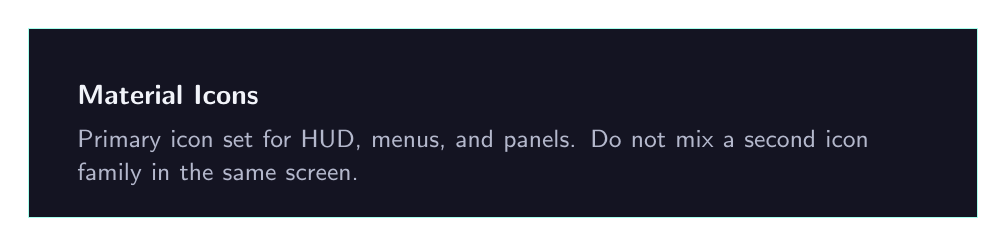
\begin{tikzpicture}
  \fill[panel] (0,0) rectangle (\textwidth-2pt,2.4);
  \draw[signal!35] (0,0) rectangle (\textwidth-2pt,2.4);
  \node[anchor=west] at (0.5,1.55) {\textcolor{ghost}{\sffamily\bfseries Material Icons}};
  \node[anchor=west, text width=0.85\textwidth] at (0.5,0.75)
    {\textcolor{muted}{\sffamily\small Primary icon set for HUD, menus, and panels. Do not mix a second icon family in the same screen.}};
\end{tikzpicture}

\clearpage

% =====================================================================
% 6. DELIVERABLE
% =====================================================================
\section*{06 · Filformat}
\addcontentsline{toc}{section}{Filformat}

\begin{itemize}
  \item \textbf{Required format:} PDF
  \item \textbf{This file:} \texttt{docs/brand/echoes\_of\_elysium\_graphical\_profile.pdf}
  \item \textbf{Source:} \texttt{docs/brand/echoes\_of\_elysium\_graphical\_profile.tex}
  \item \textbf{Build:} \texttt{xelatex echoes\_of\_elysium\_graphical\_profile.tex}
\end{itemize}

\vspace{1.2em}
\begin{center}
\textcolor{signal!55}{\rule{8cm}{0.65pt}}\\[0.65em]
{\sffamily\textcolor{ghost}{Echoes of Elysium — graphical profile v2.0}}\\[0.35em]
{\labelfont\small\textcolor{signal}{END · KEEP NEXT TO THE BUILD}}
\end{center}

\end{document}
